\section{Análisis Orientado a Objetos}
Se describen a continuación las tres etapas generales en que se divide el análisis orientado a objetos bajo la metodología OMT++. Cada etapa se contruye a partir de una etapa anterior o de las especificaciones de casos de uso obtenidos durante la creación del avance anterior.

El análisis de objetos consiste en la especificación de los conceptos clave relacionados al sistema siendo desarrollado. A partir de un análisis de las descripciones de casos de uso se produce un "modelo de objetos" siguiendo las normas del lenguaje unificado de modelado o UML.

En la etapa de análisis de compotamiento se definen las operaciones realizadas por el usuario para la manipulación e ingreso de información, sin especificar detalles de la interfaz. Este artefacto recibe el nombre de "lista de especificación de operaciones" y se crea con el objetivo de que el sistema final puedo ejecutar todas las operaciones contenidas en dicha lista. Similar a la etapa anterior, gran parte de del trabajo realizado en esta etapa consiste en el análisis de responsabilidad del usuario dentro de las descripciones de los casos de uso en el avance anterior.

\subsection{Análisis de Objetos}
Durante el análisis de objetos se utilizan los resúmenes de los casos de uso detalladas en el avance anterior. A partir de estos se han indentificado las posibles clases para el modelo de objetos de análisis. Se considera cada caso de uso para luego evaluar modelos apropiados al sistema a desarrollar.

\subsubsection{Modelo de Objetos de Análisis}
\begin{figure}[H]
	\centering
	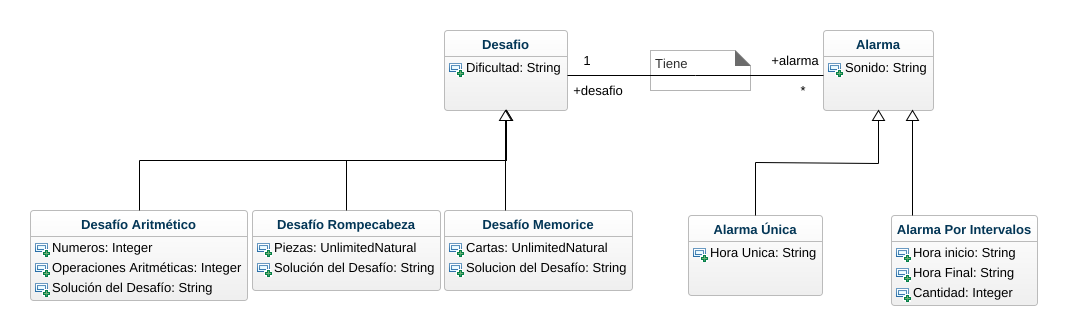
\includegraphics[page=1,width=\textwidth]{./img/uml.png}
	\caption{Diagrama de Objetos de Análisis}
        \vspace{10pt}
	\label{fig:Diagrama de Objetos de Análisis}
\end{figure}

\subsubsection{Diccionario de Datos del Modelo de Objetos}
\begin{table}[H]
    \centering
    \caption{Diccionario de Datos}
    \vspace{10pt}
    \begin{tabular}{|l|p{0.4\linewidth}|p{0.4\linewidth}|}
        \hline
        \textbf{Clase} & \textbf{Descripción} & \textbf{Atributos} \\
        \hline
        Desafío & Desafío a resolver & Dificultad: nivel de dificultad\\
        \hline
        Desafío Aritmético & Desafío que requiere la resolución de problemas aritméticos & Números: número de operandos\newline Operaciones Aritméticas: operadores a utilizar\newline Solución: solución del desafío\\
        \hline
        Desafío Rompecabezas & Desafío que requiere la resolución de un rompecabezas. & Piezas: número de piezas a organizar \newline Solución: orden correcto de las piezas\\
        \hline
        Alarma & Una alarma o grupo de alarmas fijadas. & Sonido: sonido a utilizar\\
        \hline
        Alarma Única & Alarma que no pertenece a un grupo. & Hora: hora de activación de la alarma\\
        \hline
        Alarma Por Intervalo & Grupo de alarmas que sonarán durante un intervalo de tiempo. & Hora Inicio: hora de la primera alarma\newline Hora Final: hora de la última alarma\newline Cantidad: número de alarmas que sonarán durante el intervalo.\\
        \hline

    \end{tabular}
    
    \label{table:1}
\end{table}


\subsection{Análisis de Comportamiento}
Se utilizan los casos de uso definidos anteriormente para crear la lista de operaciones. A partir de la descripción de flujo normal para dichos casos se definen las operaciones realizadas por el usuario, identificando todos los casos de uso donde se repiten.

\subsubsection{Especificación de Operaciones}
Se listan a continuación todas las operaciones identificadas a partir de los casos de uso.
\begin{table}[H]
    \centering
    \caption{Lista de Operaciones de Usuario}
    \vspace{5pt}
    \begin{tabular}{| c | l | l |}
        \hline
        Número & Operación & ID Caso de Uso \\
        \hline
        1 & Ingresar hora de inicio & 1 - 12 \\
        \hline
        2 & Ingresar hora de término & 1 - 12 \\
        \hline
        3 & Ingresar frecuencia & 1 - 12 \\
        \hline
        4 & Seleccionar opción ``Desafío aritmético" & 1 - 2 - 10 - 12 - 6 \\
        \hline
        5 & Seleccionar opción ``Desafío rompecabezas" & 1 - 2 - 10 - 12 - 6 \\
        \hline
        6 & Seleccionar opción ``Desafío memorice" & 1 - 2 - 10 - 12 - 6 \\
        \hline
        7 & Seleccionar opción ``Ingresar Intervalo" & 1 \\
        \hline
        8 & Ingresar hora de alarma & 2 - 10 - 6 \\
        \hline
        9 & Seleccionar opción ``Ingresar alarma" & 2 \\
        \hline
        10 & Ingresar solución & 3 \\
        \hline
        11 & Seleccionar opción ``Ingresar Solución" & 3 \\
        \hline
        12 & Mover piezas del rompecabezas & 4 \\
        \hline
        13 & Seleccionar opción ``Comprobar" & 4 \\
        \hline
        14 & Seleccionar cartas & 5 \\
        \hline
        15 & Seleccionar opción ``Desactivar alarma" & 7 \\
        \hline
        16 & Seleccionar opción ``Alarma única" & 8 \\
        \hline
        17 & Seleccionar opción ``Alarma por Intervalos" & 8 \\
        \hline
        18 & Seleccionar opción "Seleccionar alarma" & 9 \\
        \hline
        19 & Seleccionar opción "Eliminar alarma" & 8 \\
        \hline
        20 & Ingresar invervalo & 10 - 12 \\
        \hline
        21 & Seleccionar opción "Guardar cambios" & 10 - 6 - 12 \\
        \hline
    \end{tabular}    
    
    \label{table:2}
\end{table}

\subsection{Especificación de la interfaz de usuario}
En esta sección se presenta el diagrama de diálogo y la especificación de sus componentes que servirán como base para la interfaz de usuario de Snoozefest. El diagrama de diálogo representa la forma en que el usuario interactúa con el sistema y se mueve a través de los diálogos, mientras que la especificación de sus componentes establece los elementos que compondrán dichos diálogos.

\subsubsection{Diagramas de Diálogo}
El diagrama de diálogo permite visualizar claramente la interacción entre el usuario y el sistema, permitiendo visualizar las operaciones que conectan a los diálogos.
\begin{figure}[H]
	\centering
	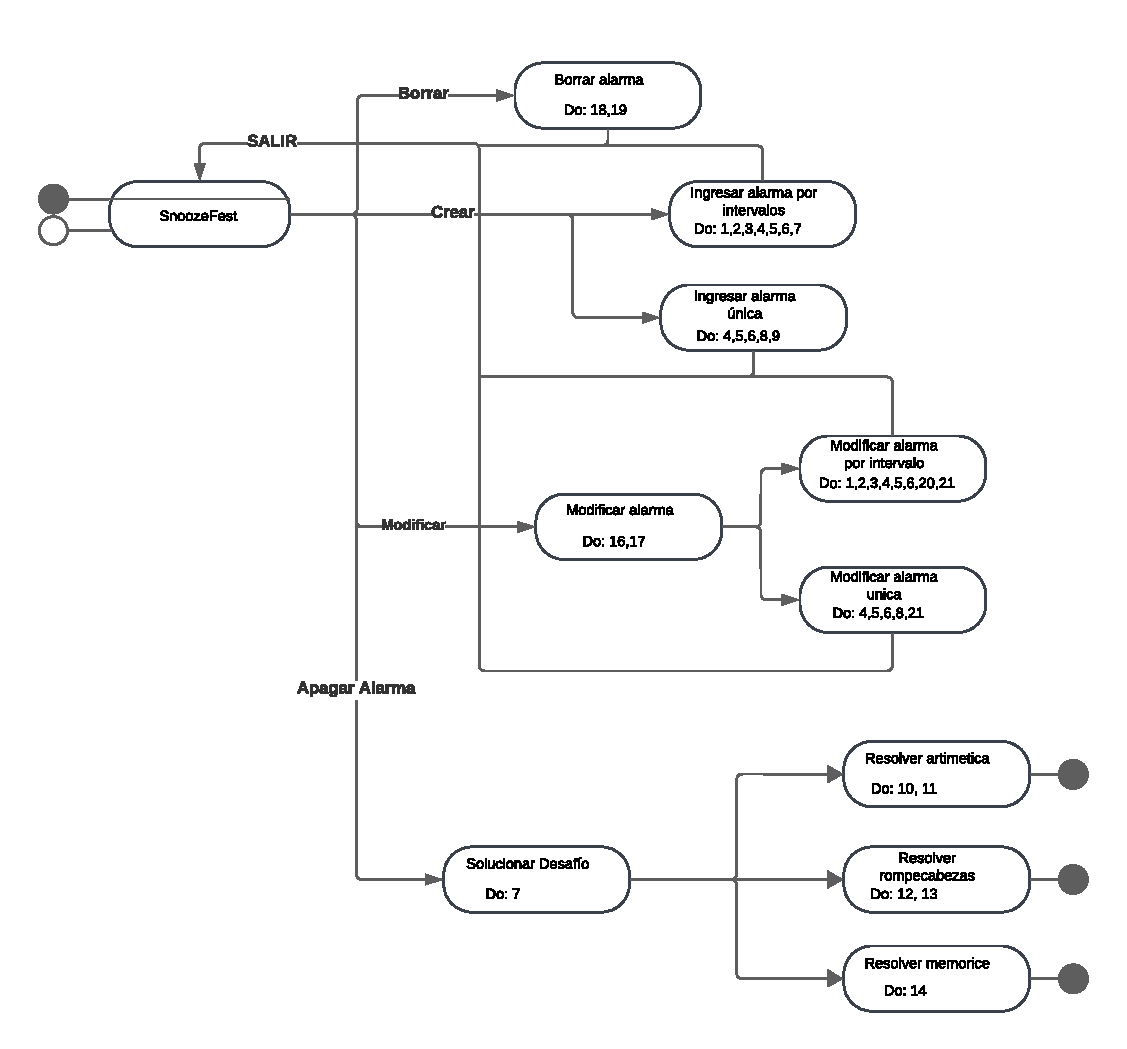
\includegraphics[page=1,width=\textwidth]{./img/dialogos.pdf}
	\caption{Diagramas de Diálogo}
        \vspace{10pt}
	\label{fig:Diagrama de Diálogos}
\end{figure}

\subsubsection{Especificación de Componentes}
Habiendo establecido los diálogos, se especifican los elementos que los componen.

\begin{figure}[H]
	\centering
	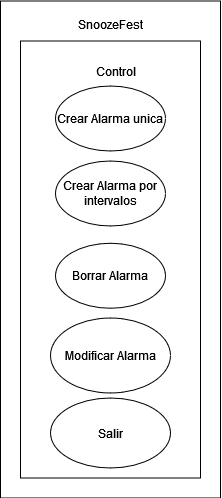
\includegraphics[width=0.3\textwidth]{~/uni/inge2/informe3/img/componentes/01-PrincipalSnoozefest.png}
	\caption{Snoozefest}
        \vspace{5pt}
	\label{fig:Snoozefest}
\end{figure}

\begin{figure}[H]
	\centering
	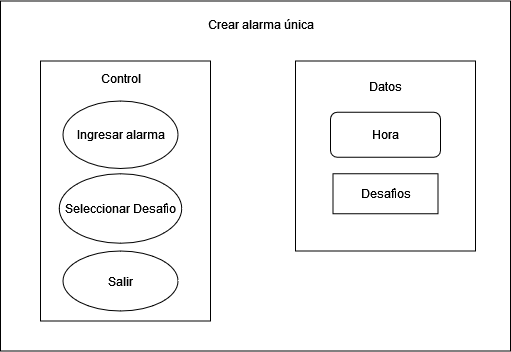
\includegraphics[width=0.5\textwidth]{~/uni/inge2/informe3/img/componentes/02-CrearAlarmaUnica.png}
	\caption{Crear Alarma Única}
        \vspace{5pt}
	\label{fig:Crear Alarma Única}
\end{figure}

\begin{figure}[H]
	\centering
	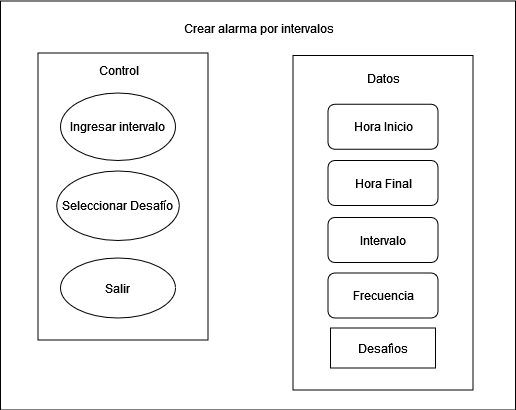
\includegraphics[width=0.5\textwidth]{~/uni/inge2/informe3/img/componentes/03-CrearAlarmaPorIntervalos.png}
	\caption{Crear Alarma por Intervalos}
        \vspace{5pt}
	\label{fig:Crear Alarma por Intervalos}
\end{figure}

\begin{figure}[H]
	\centering
	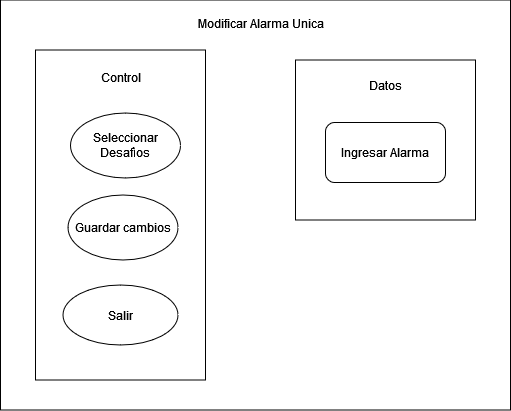
\includegraphics[width=0.5\textwidth]{~/uni/inge2/informe3/img/componentes/04-ModificarAlarmaUnica.png}
	\caption{Modificar Alarma Única}
        \vspace{5pt}
	\label{fig:Modificar Alarma Única}
\end{figure}

\begin{figure}[H]
	\centering
	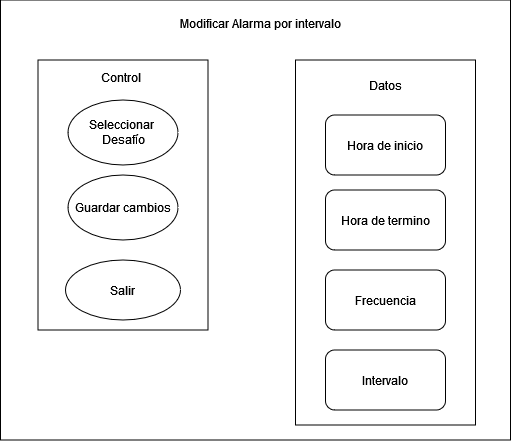
\includegraphics[width=0.5\textwidth]{~/uni/inge2/informe3/img/componentes/05-ModificarAlarmaIntervalos.png}
	\caption{Modificar Alarma por Intervalos}
        \vspace{5pt}
	\label{fig:Modificar Alarma por Intervalos}
\end{figure}

\begin{figure}[H]
	\centering
	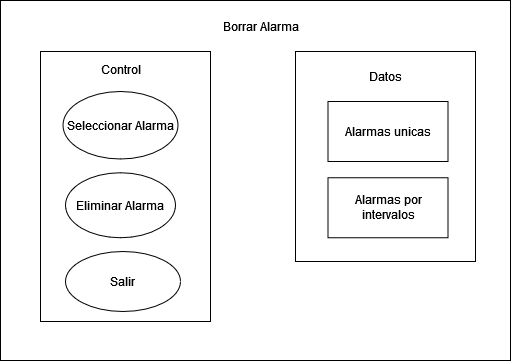
\includegraphics[width=0.5\textwidth]{~/uni/inge2/informe3/img/componentes/06-BorrarAlarma.png}
	\caption{Borrar Alarma}
        \vspace{5pt}
	\label{fig:Borrar Alarma}
\end{figure}

\begin{figure}[H]
	\centering
	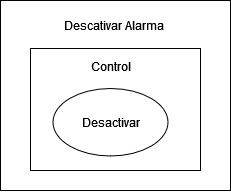
\includegraphics[width=0.5\textwidth]{~/uni/inge2/informe3/img/componentes/07-DesactivarAlarma.png}
	\caption{Desactivar Alarma}
        \vspace{5pt}
	\label{fig:Desactivar Alarma}
\end{figure}

\begin{figure}[H]
	\centering
	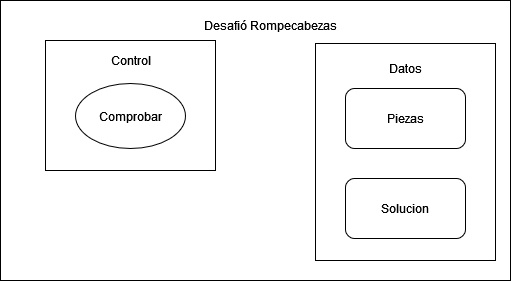
\includegraphics[width=0.5\textwidth]{~/uni/inge2/informe3/img/componentes/08-DesafioRompecabezas.png}
	\caption{Desafío Rompecabezas}
        \vspace{5pt}
	\label{fig:Desafío Rompecabezas}
\end{figure}

\begin{figure}[H]
	\centering
	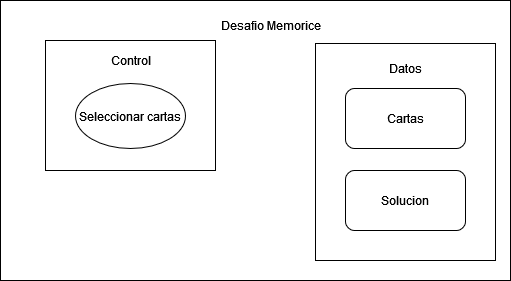
\includegraphics[width=0.5\textwidth]{~/uni/inge2/informe3/img/componentes/09-DesafioMemorice.png}
	\caption{Desafío Memorice}
        \vspace{5pt}
	\label{fig:Desafío Memorice}
\end{figure}

\begin{figure}[H]
	\centering
	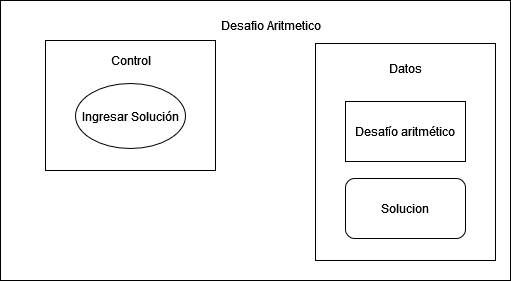
\includegraphics[width=0.5\textwidth]{~/uni/inge2/informe3/img/componentes/10-DesafioAritmetico.png}
	\caption{Desafío Aritmético}
        \vspace{5pt}
	\label{fig:Desafío Aritmético}
\end{figure}

